\documentclass[../main/main.tex]{subfiles}
\begin{document}

% \dominitoc
% \faketableofcontents
% \dominilof
% \fakelistoffigures
% \dominilot
% \fakelistoftables

\chapter{Introduction \`a \snana}\label{ch:snana}
\epigraph{\openquote\textit{A common mistake that people make when trying to
design something completely foolproof is to underestimate the ingenuity of
complete fools}\closequote}{Douglas \textsc{Adams}, \textit{Mostly Harmless}}

Nous avons vu Chapitre~\ref{ch:sne} qu'à partir de 1993, grâce la
standardisation des SNe~Ia par l'étude de leurs caractéristiques d'étirement et
de couleur notamment, la cosmologie basée sur les SNe~Ia a pu prospérer, donnant
une incertitude sur les modules de distances d'environ 15\%~; si cela était
suffisant à améliorer la précision de l'époque, dominée par les incertitudes
statistiques, la source principale d'erreur sur les mesures de paramètres
cosmologiques est depuis devenue l'incertitude systématique.

À cet effet, l'ensemble de logiciels SuperNova ANAlysis
\citep[\snana,][]{kessler2009a} tente d'homogénéiser les différentes analyses
cosmologiques par le biais d'un outil fiable aux procédures reproductibles et
aux implémentations évolutives. La versatilité de ce projet en fait un outil
largement utilisé en cosmologie \citep[par exemple,][]{kessler2009b, conley2011,
betoule2014, smith2020} que ce soit pour étudier un sondage précis ou une
combinaison de sondages. C'est donc naturellement qu'après avoir étudié
l'évolution des propriétés des SNe~Ia en corrélation avec leur environnement
Chapitre~\ref{ch:stretch}, nous nous sommes dirigæ vers ce logiciel afin
d'estimer l'impact de cette modélisation sur la détermination des paramètres
cosmologiques.

Nous présentons le paquet dans ce chapitre. Nous commençons par le contexte de
son établissement Section~\ref{sec:snanacont}, avant de détailler les deux
étapes clés de son fonctionnement~: la simulation et l'ajustement de courbes de
lumière (Section~\ref{sec:snanasim}) et la correction des biais sur la distance
et le calcul des paramètres cosmologiques (Section~\ref{sec:biais}).

\vfill
\minitoc
\vfill

\newpage

\section{Contexte}\label{sec:snanacont}

C'est dans le contexte de la diversité des analyses cosmologiques,
particulièrement la diversité de logiciels d'ajustement de courbes de lumière,
que le paquet \snana\ a vu le jour \citep{kessler2009a}. Son objectif est de
fournir aux différents groupes un outil public et fiable permettant la
reproductibilité des analyses. C'est un ensemble de logiciels, incluant un
ajusteur de courbes de lumière, un simulateur Monte Carlo, et un ajusteur de
cosmologie, simulant des catalogues de données\footnote{une autre approche
    pourrait simuler des images, mais ceci augmenterait exponentiellement le
temps de calcul}. Les logiciels intègrent des modèles existants mais offrent
également la possibilité de s'adapter à de nouveaux modèles, ne se limitant
pas qu'aux SNe~Ia (il y a par exemple des modèles de Kilo Novae) et
admettant depuis des corrélations entre une SN et son environnement,
devenues aussi importantes que la qualité d'ajustement comme discuté
Chapitre~\ref{ch:env}.

En effet, la décennie passée a vu de nombreux efforts être dirigés vers
l'implémentation de simulations de qualités pour corriger les biais dépendant du
redshift du module de distance ayant pour cause les effets de sélections, et
\snana\ établit un cadre d'étude permettant de simuler ces effets pour
différents sondages \citep{kessler2019}. Ces effets peuvent être d'origines
variées~: de la magnitude limite des instruments causant du biais de
\textsc{Malmquist}, comme présenté Chapitre~\ref{ch:sample}, mais aussi de la
qualité des procédures de détection de phénomènes transitoires, de choix de
candidats pour le suivi spectro-photométrique ou des critères de sélection des
données considérées comme valables cosmologiquement (voir
Chapitre~\ref{ch:surveys}). Les Figures~4 à 7 du Chapitre~\ref{ch:sample} sont
en effet tirées de simulations, et indiquent un biais pouvant aller jusqu'à
\SI{0.10}{mag}. Enfin, les biais sur le module de distance dépendent également
des populations mères de l'étirement et de la couleur d'une SN~Ia mais aussi des
variabilités intrinsèques de magnitude~: c'est cette partie spécifiquement qui
est à l'étude dans notre thèse.

Nous pouvons résumer son fonctionnement à trois étapes clés~: (1) la simulation
d'une courbe de lumière de SN~Ia et (2) son ajustement, regroupées dans la
Section~\ref{sec:snanasim}), et (3) un ajuster de cosmologie \textit{via} la
dérivation de la distance des SNe~Ia (Section~\ref{sec:biais}).

\section{Simulation}\label{sec:snanasim}

Nous présentons dans cette section les étapes-clés des simulations avec \snana\
(dont le pipeline est automatisé par \texttt{PIPPIN} \citep{hinton2020}), telles
que nous les effectuons. Dans la Section~\ref{ssec:simprep} nous introduisons
les concepts fondamentaux régissant le fonctionnement du logiciel~; les étapes
successives de génération (Section~\ref{ssec:simsn}), réponse instrumentale
(Section~\ref{ssec:siminst}) et de détection (Section~\ref{ssec:simdetec})
viennent ensuite. Un résumé est proposé Section~\ref{ssec:simshort}, avec la
Figure~\ref{fig:snana_func}.

\subsection{Préparation d'une simulation}\label{ssec:simprep}

Les simulations avec \snana\ reposent sur deux librairies principales~: (1) une
librairie de galaxies hôtes (\hostlib) décrivant le lien entre une SN et son
environnement, et (2) une librairie des caractéristiques instrumentales d'un
télescope (\simlib) reproduisant les observations d'un sondage et leurs
conditions de relevé. Dans notre approche de la manière dont nos simulations
fonctionnent, ces librairies précèdent le procédé de simulation.

\subsubsection{\hostlib}\label{sssec:hostlib}

D'une manière générale, chaque galaxie de la \hostlib\ est décrite par~:
\begin{enumerate}
    \item Un numéro d'identification (\texttt{GALID})~;
    \item Une position de son centre dans le ciel \textit{via} la donnée
        d'ascension droite (\texttt{RA\_GAL}) et de déclinaison
        (\texttt{DEC\_GAL})~;
    \item Un redshift photométrique ($z_{\rm TRUE}$)~;
    \item Ses magnitudes dans les différentes bandes photométriques ($grizY_{\rm
        obs}$)~;
    \item Un profil de \textsc{Sérsic} (décrivant l'évolution de son intensité
        avec la distance $R$ de son centre)~;
    \item Une masse en échelle logarithmique en masses solaires
        (\texttt{LOGMASS}) et son erreur (\texttt{LOGMASS\_ERR}).
\end{enumerate}
Ces caractéristiques permettent, lors de la simulation d'une supernova, de la
placer à une position autour du centre galactique selon le profil de
\textsc{Sérsic} afin de déterminer la luminosité de surface locale et d'ajouter
un bruit Poissonnien aux courbes de lumières qui suivront \citep{kessler2019}.
Dans notre cas le plus complexe, la \hostlib\ présente également les
caractéristiques qu'une SN de cette galaxie hôte doit respecter~:
\begin{enumerate}[resume]
    \item Sa couleur \texttt{C}~;
    \item Son étirement \texttt{X1}~:
    \item Son âge \textit{via} le \texttt{LSSFR}~;
    \item La marche de magnitude associée \texttt{SNMAGSHIFT} (voir
        Chapitre~\ref{ch:env}).
\end{enumerate}
La \hostlib\ apparaît donc, dans notre cadre d'étude, comme l'élément clé
permettant de faire varier les distributions sous-jacentes des paramètres des
SNe~Ia. Nous décrivons la réalisation de celle-ci et les différentes
implémentations de \hostlib\ Chapitre~\ref{ch:sims}~; pour le moment nous nous
contentons de décrire sa construction par l'utilisation de distributions des
paramètres de couleur et d'étirement générant ladite table. Cette étape est
représentée dans le cadre supérieur gris de la Figure~\ref{fig:snana_func}, et
un extrait d'une de nos \hostlib\ est donné Figure~\ref{fig:nrenv}.

\begin{figure}[]
    \centerfloat
    \VerbatimInput[fontsize=\fontsize{8pt}{10pt}\selectfont,
        frame=single,  % whole frame around fiure
        framesep=1em,  % separation between frame and text
        %boxwidth=1.5\linewidth,
        label=\fbox{\fontsize{10pt}{12pt}\selectfont NR\_highz.HOSTLIB},
        labelposition=topline]{../data/NR_highz.HOSTLIB}
        \caption[Extrait d'une \hostlib\ utilisée dans notre étude]{Extrait
        d'une \hostlib\ utilisée dans notre étude, modifiée pour l'exemple.}
    \label{fig:nrenv}
\end{figure}

\subsubsection{\simlib}\label{sssec:simlib}

La \simlib, de son côté, présente pour chaque champ d'observation~:
\begin{enumerate}
    \item son nom (par exemple, 82N dans la Figure~\ref{fig:sdssimlib})~;
    \item ses coordonnées \texttt{RA} et \texttt{DECL}~;
    \item le nombre d'observations \texttt{NOBS}~;
    \item son extinction galactique \texttt{MWEBV}~;
    \item la taille d'un pixel \texttt{PIXSIZE}.
\end{enumerate}
et pour chaque observation~:
\begin{enumerate}[resume]
    \item la date d'observation exprimée en jours julien modifié \texttt{MJD}
        associée à un identifiant \texttt{IDEXPT}~;
    \item le filtre concerné par l'observation (\texttt{FLT})~;
    \item les caractéristiques de la caméra CCD\footnote{\textit{charged coupled
        device}, un capteur photographique} (\texttt{CCD GAIN} et \texttt{CCD
        NOISE}) au moment de l'acquisition~;
    \item le bruit dû à l'atmosphère \textit{via} le paramètre \texttt{SKYSIG}
        donnant le bruit par pixel, sommé sur l'ouverture effective dérivée par
        un ajustement de \textit{Point Spread Function} (PSF) par les données
        \texttt{PSF1}, \texttt{PSF2} et \texttt{PSF2/1} \citep[voir Section~2
        de][pour les détails]{kessler2009a}~;
    \item le point zéro moyen \texttt{ZPTAVG} et son erreur \texttt{ZPTERR}
        permettant de convertir la magnitude observée $m$ en flux $F$ en
        comptages de photons arrivant sur une CCD \textit{via} la relation $F =
        10^{-0.4(m-\texttt{ZPTAVG})}$.
\end{enumerate}
En plus de ces données, d'autres caractéristiques comme les périodes de
non-observation ou les corrections de flux à ajouter pour suivre la calibration
des télescopes sont indiquées. La Figure~\ref{fig:sdssimlib} présente un extrait
de la \simlib\ du télescope de SDSS.

\begin{figure}[ht]
    \centering
    \begin{minipage}{0.75\linewidth}
        \VerbatimInput[fontsize=\fontsize{8pt}{10pt}\selectfont,
            frame=single,  % whole frame around fiure
            framesep=1em,  % separation between frame and text
            label=\fbox{\fontsize{10pt}{12pt}\selectfont SDSS.SIMLIB},
            labelposition=topline]{../data/SDSS.SIMLIB}
    \end{minipage}
    \caption[Extrait de la \simlib\ de SDSS]{Extrait de la \simlib\ de SDSS.
    Données de~\cite{kessler2013}.}
    \label{fig:sdssimlib}
\end{figure}

En plus de ces librairies, à chaque sondage est associée une carte de poids
(\wgtmap), qui servira à pondérer la \hostlib\ sur le paramètre de masse de
manière à ce que les galaxies auxquelles sont reliées les SNe~Ia correspondent à
la distribution des masses de galaxies hôtes effectivement observée par le
sondage. Un exemple est indiquée sous le titre encadré \wgtmap\ dans la
Figure~\ref{fig:snana_func}. Cette librairie a une importance capitale depuis
l'inclusion de la masse de l'hôte comme traceur environnemental des propriétés
sous-jacentes des SNe~Ia (voir Chapitre~\ref{ch:env}). En effet, lorsqu'une
\hostlib\ n'inclut pas de marche de magnitude, c'est la \wgtmap\ qui ajoute aux
galaxies de $M_* < 10^{10}\si{\Msun}$ une variation de magnitude de
\SI{0.025}{mag} et à celles de $M_* > 10^{10}\si{\Msun}$ une variation de
\SI{-0.025}{mag} pour correspondre aux observations de marche de magnitude
basées sur la masse.

La simulation d'une supernova suit ensuite 3 étapes majeures, décrites
dans~\cite{kessler2019}~:
\begin{enumerate}
    \item Génération de la source et application d'effets cosmologiques,
        simulant la propagation de sa lumière de son origine au haut de
        l'atmosphère~;
    \item Simulation de la réponse instrumentale selon le sondage (par exemple
        conversion de la magnitude en flux de photons captés par une caméra CCD,
        bruit de l'instrument…)~;
    \item Simulation de la détection, incluant les critères pour que la SN soit
        un candidat à l'observation (voir Chapitre~\ref{ch:surveys}) et
        l'efficacité spectroscopique du sondage.
\end{enumerate}

\subsection{Génération du modèle}\label{ssec:simsn}

Nous utilisons le modèle spectral \texttt{SALT2} de~\cite{guy2007} et
précédemment décrit Chapitre~\ref{ch:sne} pour générer une SN~Ia. Il est
initialisé dans un référentiel au repos pour des époques entre \SI{20}{jours}
avant et $\approx\SI{70}{jours}$ après le maximum d'émission. À chaque SN est
donc associé un redshift ($z_{\rm CMB}$ dans le référentiel du fonds diffus
cosmologique) à partir d'un modèle de taux de SNe~Ia (différent selon le
sondage), un maximum d'émission $t_0$ choisi au hasard sur une plage avant et
après la période d'observation de sondage, et une valeur d'étirement $x_1$ et de
couleur $c$. Notre approche est d'effectuer un tirage des ces paramètres depuis
la \hostlib, pondérée par la \wgtmap\ du sondage, en faisant correspondre le
redshift choisi initialement avec une des entrées de la table. Ce tirage donne
également la valeur de la marche de magnitude à appliquer. C'est de cette
manière que la génération du modèle est rendue dépendante de son environnement.
Cette étape est imagée par la partie «~Tirage~» (en rose) de la
Figure~\ref{fig:snana_func}, considérée comme l'étape d'entrée dans une
simulation et numérotée «~1~», menant aux paramètres de la \hostlib\ illustrée
dans la partie «~Création \hostlib~» (numérotée «~2~») par une flèche pointillée
rose étiquetée «~Lien avec l'environnement~». L'attribution de ces deux
paramètres varie selon les postulats de corrélations que nous avons implémentés,
nous y reviendrons au chapitre suivant.

Avec le redshift choisi, à cette étape est définit un module de distance réel,
$\mu_{\rm vrai}$, \textit{via} sa définition (donnée Chapitre~\ref{ch:sne}), en
supposant une cosmologie sous-jacente. Dans notre cas, nous utilisons le modèle
$w$CDM avec valeurs définies dans le Tableau~\ref{tab:cosmoinput}.

\begin{table}[ht]
    \centering
    \caption[Valeur des paramètres cosmologiques utilisés pour la détermination
    du module de distance réel de la SN simulée]{Valeur des paramètres
        cosmologiques utilisés pour la détermination du module de distance réel
    de la SN simulée.}
    \label{tab:cosmoinput}
    \begin{tabular}{ccccc}
        \toprule
        $H_0$ & $\Omega_M$ & $\Omega_\Lambda$ & $w_0$ \\
        \midrule
        \SI{70.0}{km.Mpc^{-1}.s^{-1}} & \num{0.315} & \num{0.685} & \num{-1.00}\\ 
        \bottomrule
    \end{tabular}
\end{table}

En utilisant les autres paramètres choisis, nous avons également~:
\begin{equation}\label{eq:mutrue}
    \mu_{\rm vrai} = m_{B, \rm vrai} - M + \alpha_{\rm ref} x_{1, \rm vrai} -
    \beta_{\rm ref} c_{\rm vrai}+ \gamma_{\rm env}
\end{equation}
où $\alpha_{\rm ref}$ et $\beta_{\rm ref}$ sont les coefficients des
corrélations linéaires magnitude-étirement et magnitude-couleur, respectivement
(voir Chapitre~\ref{ch:sne}). Dans cette équation, leurs valeurs sont fixées à
\num{0.145} et \num{3.1}, respectivement, suivant l'analyse
de~\cite{popovic2021a}. $M$ est également fixé, à \SI{-19.3}{mag}. La marche de
magnitude $\gamma_{\rm env}$ varie selon la source de la corrélation à
l'environnement~: pour une corrélation avec la masse $M_*$ de la galaxie hôte,
$\gamma_{\rm env} = \pm \SI{0.025}{mag}$ pour $M_* > 10^{10}\si{\Msun}$ et $M_*
< 10^{10}\si{\Msun}$ respectivement~; pour une corrélation avec l'âge de la SN,
$\gamma_{\rm env} = \pm \SI{0.065}{mag}$ pour les SNe~Ia jeunes et vieilles,
respectivement. De cette manière, nous pouvons déduire la valeur de $m_{B, \rm
vrai}$ de la magnitude apparente.

Le modèle se voit ensuite appliquer des effets de dispersion intrinsèque (dans
notre cas celui décrit dans~\cite{guy2010}, nommé
G10\defcitealias{guy2010}{G10}), de lentillage faible, de redshift pour le
placer dans le référentiel héliocentrique, et d'extinction galactique de la Voie
Lactée, appliqués à $m_{B, \rm vrai}$. Ces différents effets mènent à simuler
une magnitude en haut de l'atmosphère, avant qu'un instrument ne l'acquiert. Les
détails de ces procédures sont développés dans~\cite{kessler2019}. Cette partie
est illustrée par la flèche pointillée bleue étiquetée «~Génération~» allant de
la partie «~Création \hostlib~» numérotée «~2~» à la représentation d'une série
temporelle théorique d'une SN au début de la partie «~Instrument~» en bleu,
numérotée «~3~».

\subsection{Réponse instrumentale}\label{ssec:siminst}

Une fois les séries temporelles du spectre de la SN formées, le programme simule
le flux effectivement reçu et le bruit mesurés par le télescope du sondage
reproduit. Comme décrit dans la Section~\ref{ssec:simprep}, celle-ci est fixée
par les journaux d'observation du sondages résumés dans la \simlib. Elle permet
d'appliquer les qualités d'observation du télescope à chaque époque de la série
temporelle, mimant l'acquisition ou non des points photométriques par les bandes
optiques de l'instrument et menant à l'établissement d'une courbe de lumière.
Cette étape est représentée dans la partie «~Instrument~» en bleu dans la
Figure~\ref{fig:snana_func}, numérotée «~3~». C'est également dans cette partie,
mais non représentée sur la figure, qu'un bruit Poissonnien est ajouté à la
mesure selon la luminosité de surface locale induite par la position de la SN
par rapport au centre de sa galaxie hôte. Ces étapes simulent la transformation
du signal en haut de l'atmosphère au signal effectivement reçu sur Terre.

D'après l'auteur du paquet dans~\cite{kessler2019}, les simulations \snana\ sont
idéalement adaptées pour les sondages à recherche glissante pour lesquelles le
même instrument sert à la détection et à la mesure de courbes de lumière, par
exemple les sondages PS1, SDSS et SNLS que nous avons présentés
Chapitre~\ref{ch:surveys}~; à l'inverse, l'échantillon LOWZ (voir
Section~\ref{sec:lowz}), qui est à la fois une recherche ciblée et qui repose
sur des suivis de programmes de recherche indépendants, n'a pas de journaux de
données de recherche permettant une simulation idéale, et requiert donc des
approximations et des suppositions supplémentaires. Pour plus de détail sur ces
deux paragraphes, voir Section~6 de~\cite{kessler2019}.

\subsection{Sélection et ajustement}\label{ssec:simdetec}

Comme décrit dans le Chapitre~\ref{ch:surveys}, chacun des sondages de SNe~Ia
observant le ciel acquiert des images successives à la recherche d'événements
transitoires, mais ne déclenche l'acquisition continue et le suivi d'un candidat
uniquement si sa courbe de lumière respecte certains critères. Cette étape est
incluse dans le procédé de simulations de \snana, et comprend le rapport signal
sur bruit des données (SNR) et le nombre de détections relativement au pic
d'émission ($T_{\rm rest}$) que chaque sondage requiert dans sa recherche.
Enfin, l'efficacité spectroscopique en fonction de la magnitude est simulée en
amont de la simulation, \textit{via} l'utilisation de fausses données de SN, et
est utilisée pour effectuer la sélection des données.

La partie d'ajustement des données détectées est également faite avec
\texttt{SALT2} et n'est donc pas détaillée une nouvelle fois ici, mais tout un
stage de \snana\ y est consacré. De manière succincte, cet ajustement extrait
les paramètres $m_B$, $x_1$, $c$ et $t_0$ à partir des courbes de lumières
passant les critères de détection. $m_B$ correspond à la magnitude de la SN,
$x_1$ à son étirement, $c$ à sa couleur et $t_0$ au temps de maximum de
luminosité. À partir de leurs valeurs, une coupe supplémentaire est effectuée
pour ne conserver que les données de qualité cosmologiques, notamment devant
vérifier $-3 < x_1 < 3$~; les autres SNe~Ia ne passeront pas la sélection sur
l'ajustement et resteront au stade de détection.

Cette étape est imagée dans l'encadré «~Sélection~» en vert numéroté «~4~» dans
la Figure~\ref{fig:snana_func}, où nous avons différencié les SNe qui possèdent
des qualités cosmologiques de celles uniquement détectées
mais rejetées à l'étape suivante par des cadres orange et vert, respectivement,
accompagnés des étiquettes «~Ajustement conservé~» et «~Détection rejetée~»,
respectivement.

\subsection{Résumé}\label{ssec:simshort}

En partant de tables de \hostlib, \simlib, \wgtmap\ et d'efficacité
spectroscopique, nous décrivons ainsi les étapes d'une simulation dans l'ordre
suivant correspondants aux numéros des encadrés de la
Figure~\ref{fig:snana_func}~:
\begin{enumerate}
    \item Sélection d'un redshift à partir d'un modèle de taux de SNe~Ia~;
    \item Correspondance avec une galaxie hôte de la \hostlib\ pondérée par une
        \wgtmap\ et génération du modèle avec les paramètres d'étirement et de
        couleur correspondants~;
    \item Simulation de la réponse instrumentale menant à la courbe de lumière~;
    \item Application des critères de détection et de sélection des données~;
    \item Conservation des données passant les précédentes étapes.
\end{enumerate}
Sur la figure, la distribution des redshifts provient de l'Équation~6
de~\cite{perrett2012} avec les valeurs de~\cite{popovic2021a} se basant sur
l'étude de~\cite{scolnic2018}~:
\begin{equation}
    \mathrm{SNR}_{\rm Ia}(z) = r_0(1+z)^{\alpha}\quad\text{avec}\quad \left\{
        \begin{array}{rcl}
            r_0 & = & \SI{2.6e-5}{SNe.an^{-1}.Mpc^{-3}} \\
            \alpha & = &
            \left\{
                \begin{array}{rcl}
                    \num{2.2} & \text{pour} & \text{SDSS, PS1, SNLS}\\
                    \num{1.5} & \text{pour} & \text{LOWZ}
                \end{array}
            \right.
        \end{array}
    \right.
\end{equation}
Dans les encadrés 1, 3, 4, les graphiques utilisent les valeurs et données de
SDSS \citep{sako2018}. La \wgtmap\ et l'efficacité spectroscopique sont celles
de~\cite{popovic2021a}.

\begin{figure}[p]
    \vspace*{-3.2cm}
    \thisfloatpagestyle{empty}
    \centerfloat
    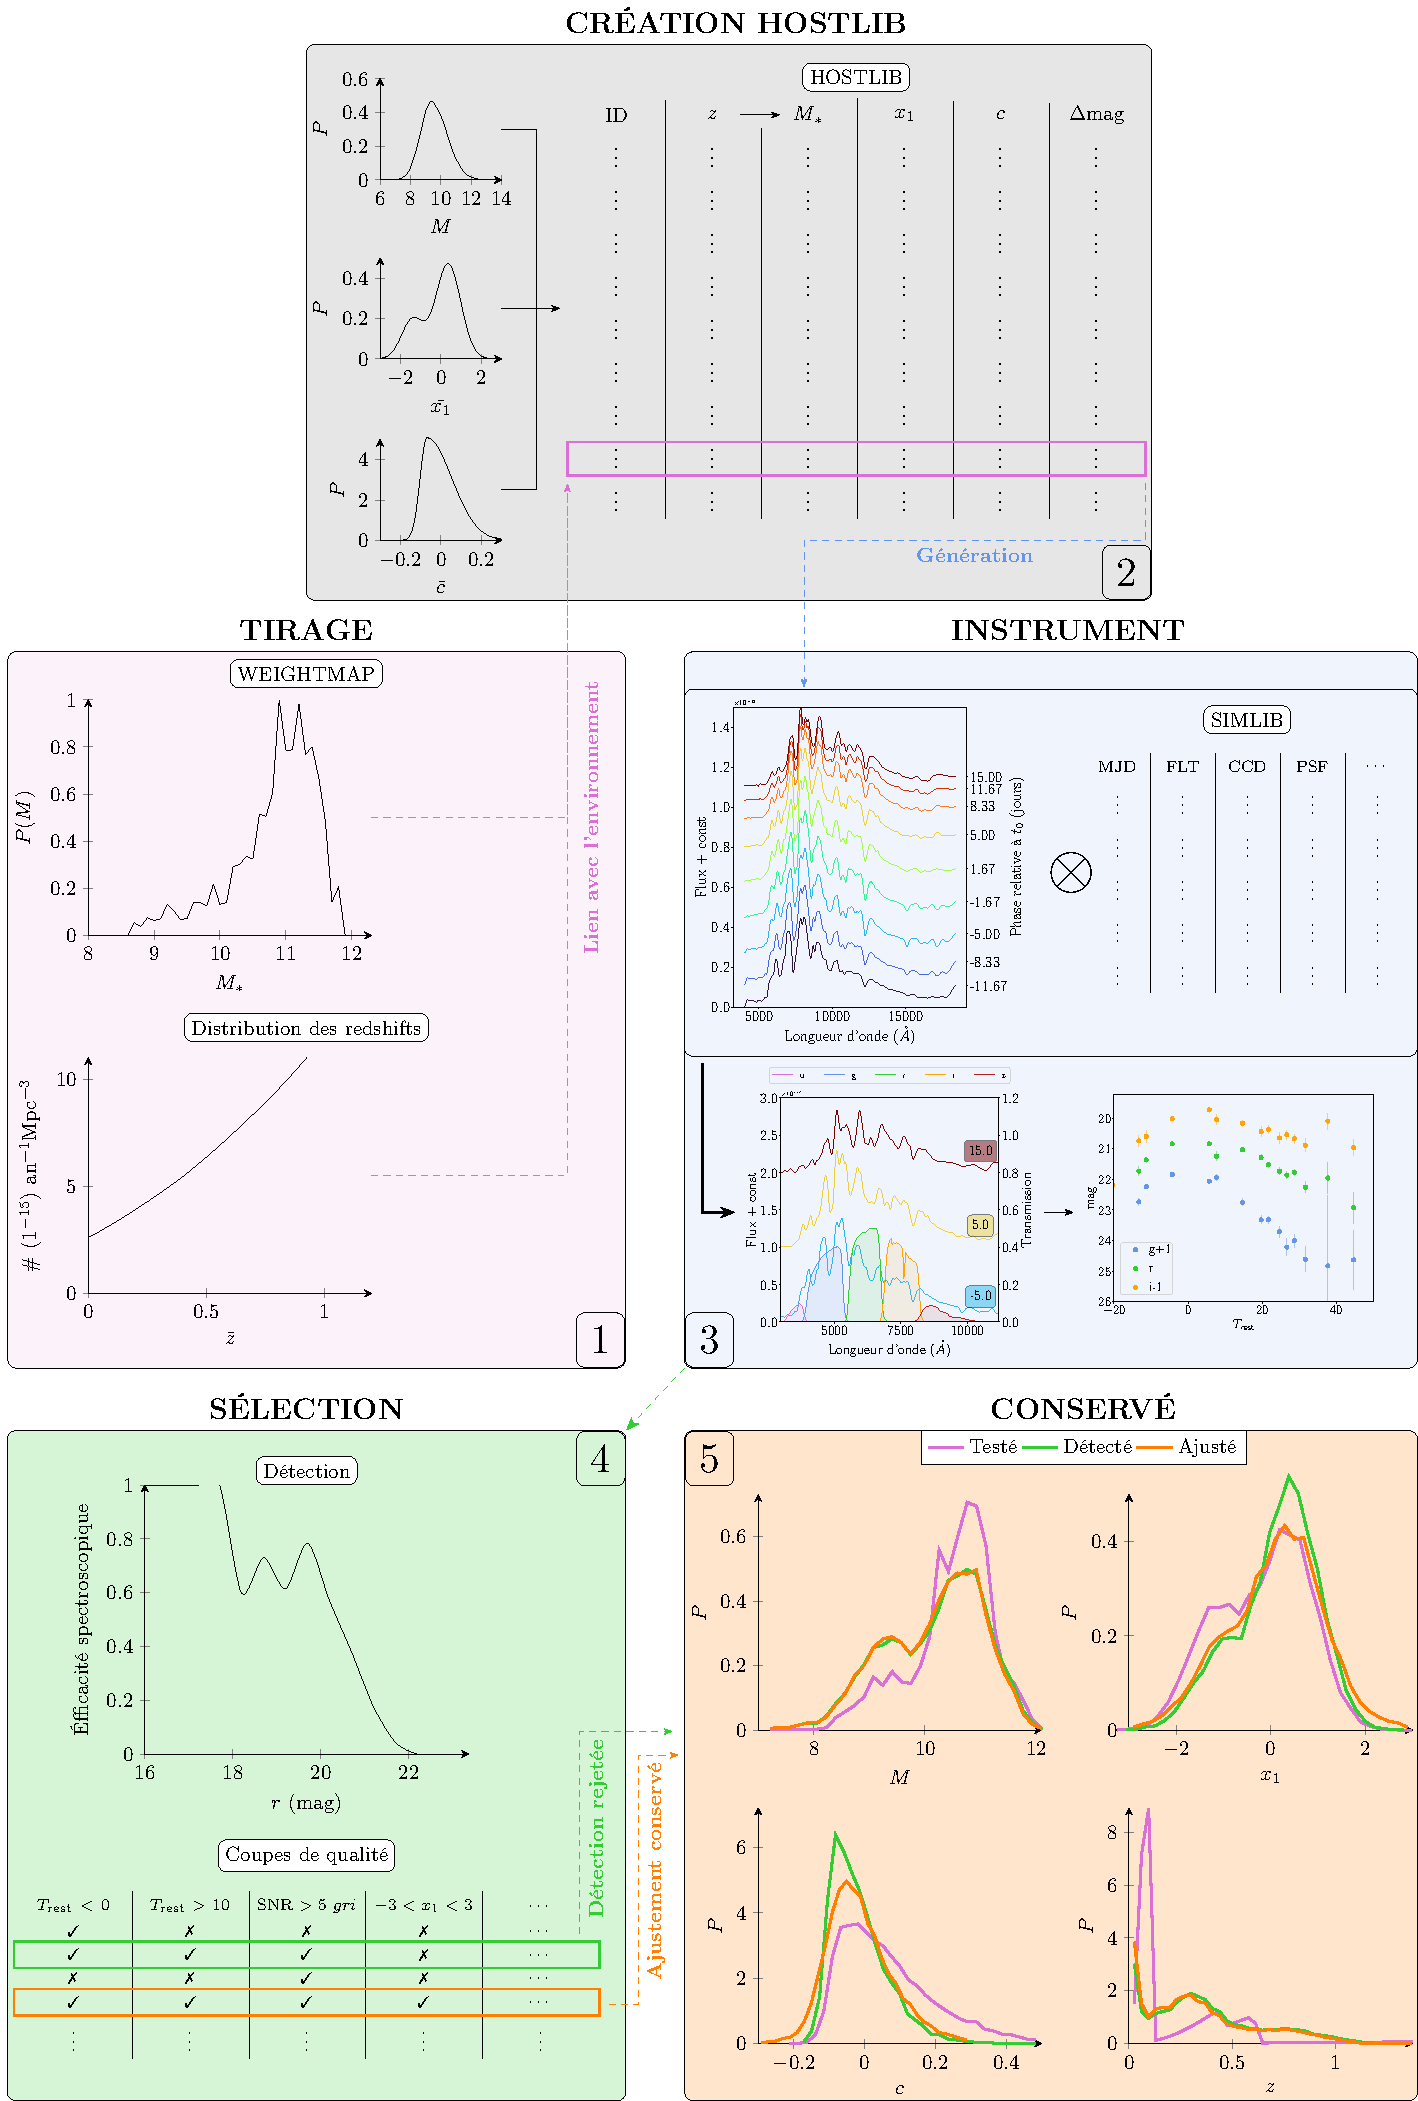
\includegraphics[width=1\linewidth]{snana_layout}
    \caption[Schéma de fonctionnement d'une simulation avec
    \snana]{\footnotesize Les tables de \wgtmap, \simlib, et de l'efficacité
        spectroscopique sont des données, ici celles du sondage SDSS. En amont
        de la simulation, une \hostlib\ est créée (\textit{en gris}, «~Création
        \hostlib~»). Pour simuler une SN~Ia, un redshift est sélectionné depuis
        une distribution (étape 1 \textit{en rose}, partie «Tirage») et est
        relié à un environnement \textit{via} un tirage la \hostlib\ pondérée
        par une carte de poids (étape 2 \textit{en gris}). À ce tirage sont
        reliées les valeurs de $x_1$ et $c$ permettant de générer une série
        temporelle de SN. Une simulation d'observation est effectuée en y
        appliquant les paramètres simulés du télescope d'un sondage grâce à une
        \simlib, donnant une courbe de lumière théorique (étape 3 \textit{en
        bleu}, partie «~Instrument~»). Cette courbe de lumière doit ensuite
        passer les critères de détection et de qualité (étape 4 \textit{en
        vert}, partie «~Sélection~»), et pourra alors être ajustée et conservée
        (orange) ou non (vert). Nous indiquons \textit{en orange} (étape 5,
        partie «~Conservé~») et pour chaque étape de ce procédé l'évolution des
        distributions de masse, étirement, couleur et redshift d'une de nos
    simulations. L'analyse se trouve Chapitre~\ref{ch:sims}}
    \label{fig:snana_func}
\end{figure}

\section{Correction de biais et cosmologie}\label{sec:biais}

Dans cette section nous présentons l'étape d'ajusteur de cosmologie avec
corrections des biais de \snana\ basé sur la méthode \textit{BEAMS with Bias
Correction} \citep[\bbc,][]{kessler2017}. BEAMS est l'acronyme de
\textit{Bayesian Estimation Applied to Multiple Species} (estimation bayésienne
appliquée à de multiples espèces), une méthode d'ajusteur établie
dans~\cite{kunz2007} visant à prendre en compte de manière réaliste la
contamination de données non-Ia dans celles des SNe~Ia qui affectent l'étude de
la cosmologie avec les SNe~Ia. Dans notre cas, nous ne simulons pas de SNe
non-Ia et ignorons les termes de vraisemblances qui y sont reliés.

\subsection{Présentation}\label{ssec:bbcintro}

Comme introduit dans la Section~\ref{ssec:simsn}, sans biais de mesure le module
de distance de la SN simulée serait $\mu_{\rm vrai}$ de
l'Équation~\ref{eq:mutrue}, et un ajustement du diagramme de \textsc{Hubble}
avec ces valeurs ne redonnerait que la cosmologie d'entrée. Avec les valeurs de
$m_B$, $x_1$, $c$ et les caractéristiques de l'environnement de l'ajustement par
\texttt{SALT2.4} qui aura passé les étapes précédentes, on aurait un module de
distance de la forme
\begin{equation}\label{eq:mu}
    \mu = m_B - M + \alpha x_1 - \beta c + \gamma_{\rm env}
\end{equation}
Un ajustement du diagramme de \textsc{Hubble} pourrait donner un décalage à ce
modèle, mais reste sous-optimal étant donné que les biais de sélection et
d'ajustement de courbes de lumière ne sont pas pris en compte. L'intérêt de
\bbc\ est d'inclure la mesure de ces biais dans le calcul du module de
distance~; ainsi la SN se voit attribuer un module de distance selon le cadre de
la méthode \bbc, définit dans \citep{popovic2021a}~:
\begin{equation}\label{eq:mucorr}
    \mu^* = m_B + \alpha x_1 - \beta c - M_{z_i} + \delta\mu_{\rm env} +
    \delta\mu_{\rm biais}
\end{equation}
où l'étoile indique une grandeur corrigée du biais.

$\delta\mu_{\rm env}$ est le biais sur la luminosité selon l'environnement de la
SN, dans notre cas une marche de magnitude basée sur la masse («~mass step~») ou
basée sur l'âge («~age step~»), de la forme
\begin{equation}
    \delta\mu_{\rm env} = \gamma_{\rm env}\times \left(1 + e^{(X_*-S)/\tau_X}
    \right)^{-1} - \frac{\gamma_{\rm env}}{2}
\end{equation}
avec $X_* = \log(M_*)$~; $S = \num{10.0}$ la valeur de la séparation hôte massif
ou non~; $\tau_X$ la largeur de la marche de magnitude~; et $\gamma_{\rm env}$
l'amplitude de la différence magnitude entre les SNe~Ia dont l'hôte est massif
($X_* > S$) ou non ($X_* < S$) pour la \textit{mass step} ou entre les SNe~Ia
vieilles ou jeunes pour la \textit{age step}. Dans nos simulations, $S$ et
$\tau_X$ sont des valeurs fixes. Le logiciel ne permettant pas encore d'utiliser
l'âge comme traceur, cette implémentation du biais dû à l'âge de l'environnement
n'est pas représentative de la réalité~; nous en discutons au chapitre suivant. 

$\delta\mu_{\rm biais}$ est la correction au module de distance. Cette mesure
s'effectue à l'aide d'un échantillon de taille conséquente, $N \approx
\num{1e6}$ SNe~Ia simulées, appelé BiasCor. Il existe différentes manières de
mesurer ce biais selon les variables avec lesquelles il est calculé, que nous
présentons dans les sections suivantes.

Les paramètres $M_{z_i}$ sont définis dans le cadre de l'ajustement par \saltmu,
défini dans~\cite{marriner2011} et utilisé dans le cadre de \bbc. Ce programme
permet d'ajuster $\alpha$ et $\beta$ sans ajustement conjoint des paramètres
cosmologiques~: ceux-ci sont d'abord fixés, puis le programme définit des
intervalles de redshifts suffisamment petits pour considérer qu'à l'intérieur de
ceux-ci les SNe~Ia sont indépendantes de la cosmologie. Les $M_{z_i}$ sont alors
les écarts de distance dans ces intervalles de redshift $z_i$, tel que $\mu =
\mu_{\rm vrai}$ lorsque les valeurs initiales de $m_B$, $x_1$ et $c$ de la
partie Génération (Section~\ref{ssec:simsn}) sont entrées à la place des valeurs
ajustées dans l'Équation~\ref{eq:mucorr}. Ce sont ces $M_{z_i}$ qui sont
utilisées pour ajuster la cosmologie. Pour l'ajustement nous partons d'un modèle
cosmologique plat $w$CDM où $\Omega_M + \Omega_{\Lambda} = 1$, pour définir
\citep{kessler2017}\footnote{l'équation du module de distance a été corrigée par
rapport à l'article, conformément à l'équation~\ref{eq:mucosmo}}~:
\begin{align}\label{eq:mumodel}
    \mu_{\text{modèle}} & = 5\log\left(\frac{d_L}{\SI{10}{pc}}\right)
                             \quad\text{avec}\\
    d_L(z,w,\Omega_M)   & = (1+z)
                            \frac{c}{H_0}
                            \int_{0}^{z} \frac{\mathrm{d} z'}{E(z')}
                            \quad\text{et}\\
    E(z)                & = \left[ \Omega_M(1+z)^3
                                 + \Omega_{\Lambda}(1+z)^{3(1+w)}
                             \right]^{1/2}
\end{align}
et \saltmu\ utilise le paquet
\texttt{MINUIT}\footnote{\href{www.cern.ch/minuit}{www.cern.ch/minuit}}
\citep{james1975} pour ajuster la quantité~:
\begin{equation}
    \chi^2_{\rm HD} = \sum_i \frac{
                          (\mu_i^* - \mu_{\text{modèle},i} - M_{z_i})^2}{
                      \sigma_{\mu,i}^2}
\end{equation}
avec $\sigma_{\mu,i}$ les incertitudes (incluant celles sur les valeurs ajustées
par \texttt{SALT2} et leurs covariances, celles dues au lentillage faible, à
l'incertitude sur le redshift et à la dispersion intrinsèque). Plutôt que
d'ajuster $\mu_{\text{modèle}}$ pour les paramètres cosmologiques, nous les
conservons aux valeurs de références (voir Tableau~\ref{tab:cosmoinput}) et ce
sont les $M_{z_i}$ qui sont ajustés. Cela permet de varier la cosmologie
sous-jacente sans répéter l'ajustement des $\alpha$ et $\beta$. Ainsi, avec ce
formalisme, $\alpha$, $\beta$, $\gamma_{\rm env}$, $M_{z_i}$ et $\sigma_{\mu}$
sont les paramètres ajustés.

L'obtention des paramètres cosmologiques s'effectue finalement à partir de ces
paramètres ajustés par le programme \wfit, donnant $w$ et $\Omega_M$. Nous
utilisons une distribution antérieure Gaussienne pour $\Omega_M$ avec une
moyenne à \num{0.315} et une largeur de \num{0.005}, et plate pour $w$ avec
comme bornes $-1,5 < w < -0,5$. Pour plus de détails sur son fonctionnement,
voir Section~5.6 de~\cite{kessler2017}.

Nous discutons maintenant des différentes implémentation de \bbc\ pour le calcul
de $\delta\mu_{\rm biais}$.

\subsection{\bbc1D}\label{ssec:bbc1D}

Originellement, il est calculé selon une seule dimension, le redshift, et
n'affecte que la magnitude à pic d'émission $m_B$. Nous appelons cette
implémentation \bbc1D. Elle se base sur des intervalles de redshift de taille
typique $< 0,1$ découpant l'échantillon BiasCor. Dans chacun de ces intervalles,
nous calculons la moyenne pondérée des événements y appartenant, et elle est
définie à une position $z_i$ également dérivée de la moyenne pondérée des
redshifts de l'intervalle. La valeur du biais $\delta\mu_{\rm biais} = -
\delta_{m_B}$ à ajouter au module de distance mesuré est alors déterminée par
une interpolation linéaire des valeurs précédentes, et nous obtenons le module
de distance corrigé~:
\begin{align}\label{eq:mu1D}
    \mu^* & = m_B^* + \alpha x_1 - \beta c - M_{z_i}
            + \delta\mu_{\rm env} \nonumber\\
          & = (m_B-\delta_{m_B}) + \alpha x_1 - \beta c - M_{z_i}
            + \delta\mu_{\rm env} \nonumber\\
          & = m_B + \alpha x_1 - \beta c - M_{z_i}
            + \delta\mu_{\rm env} + \delta\mu_{\rm biais}(z)
\end{align}
avec $m_B^*$ la magnitude corrigée suivant sa position $z$~: toutes les SNe
appartenant au même intervalle de redshift sont corrigées du même
$\delta_{m_B}$.

Ces modules de distance corrigés sont ensuite traités par \saltmu, qui renvoie
les valeurs ajustées $\alpha$, $\beta$, $\gamma_{\rm env}$, $M_{z_i}$, et
$\sigma_{\mu}$. Après cette étape, le logiciel \wfit\ ajuste les valeurs de
$M_{z_i}$ en fonction du redshift pour avoir les paramètres cosmologiques. Un
schéma de fonctionnement est donné Figure~\ref{fig:bbc1d}.

\begin{figure}[]
    \centering
    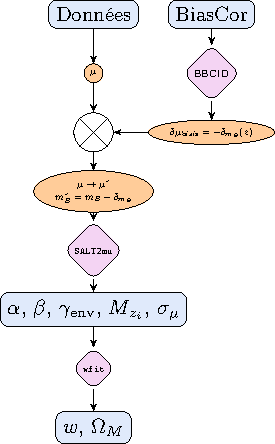
\includegraphics[scale=2]{bbc1D.pdf}
    \caption[Schéma de fonctionnement de la méthode de correction de biais de
    \bbc1D]{Schéma de fonctionnement de la méthode de correction de biais de
        \bbc\ lorsqu'elle est dans sa version à 1 dimension. De l'échantillon
        BiasCor sont déterminées les valeurs $\delta\mu_{\rm biais}$ à ajouter
        au module de distance en le découpant dans des intervalles de redshift
        pour y calculer la moyenne pondérée. Avec les données elles permettes de
        déterminer les modules de distances corrigés $\mu^*$, qui sont ensuite
        traités par \saltmu\ pour avoir les $\alpha$, $\beta$, $\gamma_{\rm
        env}$, $M_{z_i}$ et $\sigma_{\mu}$ qui permettent l'ajustement
    cosmologique par \wfit.}
    \label{fig:bbc1d}
\end{figure}

\subsection{\bbc5D}\label{ssec:bbc5D}

Développée dans~\cite{kessler2017}, cette méthode se trouve dans la prolongation
de \bbc1D, en corrigeant cette fois $m_B$, $x_1$ et $c$ à l'aide de
l'échantillon BiasCor. Plutôt que de le séquencer uniquement en redshift pour
déterminer $\delta_{m_B}$, il est divisé en cellules de tailles
$(0,05~;~0,50~;~0,05)$ respectivement. Les corrections $\delta_{m_B}$,
$\delta_{x_1}$ et $\delta_c$ à appliquer sont alors calculées de l'interpolation
des moyennes pondérées des SNe dans chacune des cellules. Nous représentons ce
procédé Figure~\ref{fig:mat}, où les exposants correspondent aux intervalles
selon $c$, $x_1$ et $z$ respectivement, pour lesquels le nombre total
d'intervalles est $C$, $X$ et $Z$, respectivement~; l'indice $p$ indique le
paramètre à sélectionner dans la cellule en question pour obtenir le biais
correspondant.

\begin{figure}[ht]
    % \vspace*{-20pt}
    \centering
    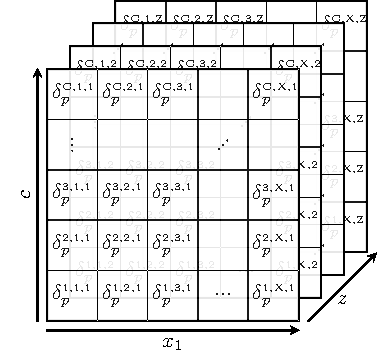
\includegraphics[width=.6\linewidth]{matrices.pdf}
    \caption[Schéma de fonctionnement du découpage de l'échantillon BiasCor en 3
    dimensions $x_1$, $c$, $z$ de la méthode \bbc5D]{Schéma de
        fonctionnement du découpage de l'échantillon BiasCor en 3 dimensions
        $x_1$, $c$, $z$ de la méthode \bbc5D. Pour une supernova dont les
        valeurs de $c$, $x_1$, $z$ sont dans les intervalles 2, 3, 1,
        respectivement, les valeurs $\delta_{m_B}$, $\delta_{x_1}$ et $\delta_c$
    seront celles issues de la cellule coloriée en vert.}
    \label{fig:mat}
\end{figure}

Avec ce découpage, on obtient cette fois~:
\begin{align}\label{eq:mu5D}
    \mu^* & = m_B^* + \alpha x_1^* - \beta c^* - M_{z_i}
            + \delta\mu_{\rm env} \nonumber\\
          & = (m_B - \delta_{m_B}) + \alpha (x_1 - \delta_{x_1}) - \beta(c-\delta_c)
            - M_{z_i} + \delta\mu_{\rm env} \nonumber\\
          & = m_B + \alpha x_1 - \beta c - M_{z_i}
            + \delta\mu_{\rm env} + \delta\mu_{\rm biais}(z, x_1, c, \alpha, \beta)
\end{align}
avec
\begin{equation}\label{eq:bias5D}
    \delta\mu_{\rm biais} \triangleq
        - \left(\delta_{m_B} + \alpha \delta_{x_1} - \beta\delta_c\right)
\end{equation}

C'est de la dimension de $\delta\mu_{\rm biais}$ que \bbc5D tire son nom. En
effet, une version 3D avec uniquement le découpage susmentionné peut exister
\citep{scolnic2016}, mais il se trouve que les valeurs de corrections de biais
dépendent des valeurs de $\alpha$ et $\beta$ utilisées. Pour reproduire cette
corrélation et étant donné que ces coefficients ont des valeurs discrètes, ces
paramètres sont générés sur une grille de taille $2\times2$, encapsulant les
valeurs trouvées par les études précédentes, et pour chacune de ces valeurs sont
définies les matrices découpées en 3D précédentes. Nous utilisons $\alpha =
[0,10~;~0,20]$ et $\beta = [2,8~;~3,4]$ (étant donné que notre dispersion
intrinsèque est basée sur~\citetalias{guy2010}). Nous illustrons ce principe
Figure~\ref{fig:mat5D}.

\begin{figure}[ht]
    \centering
    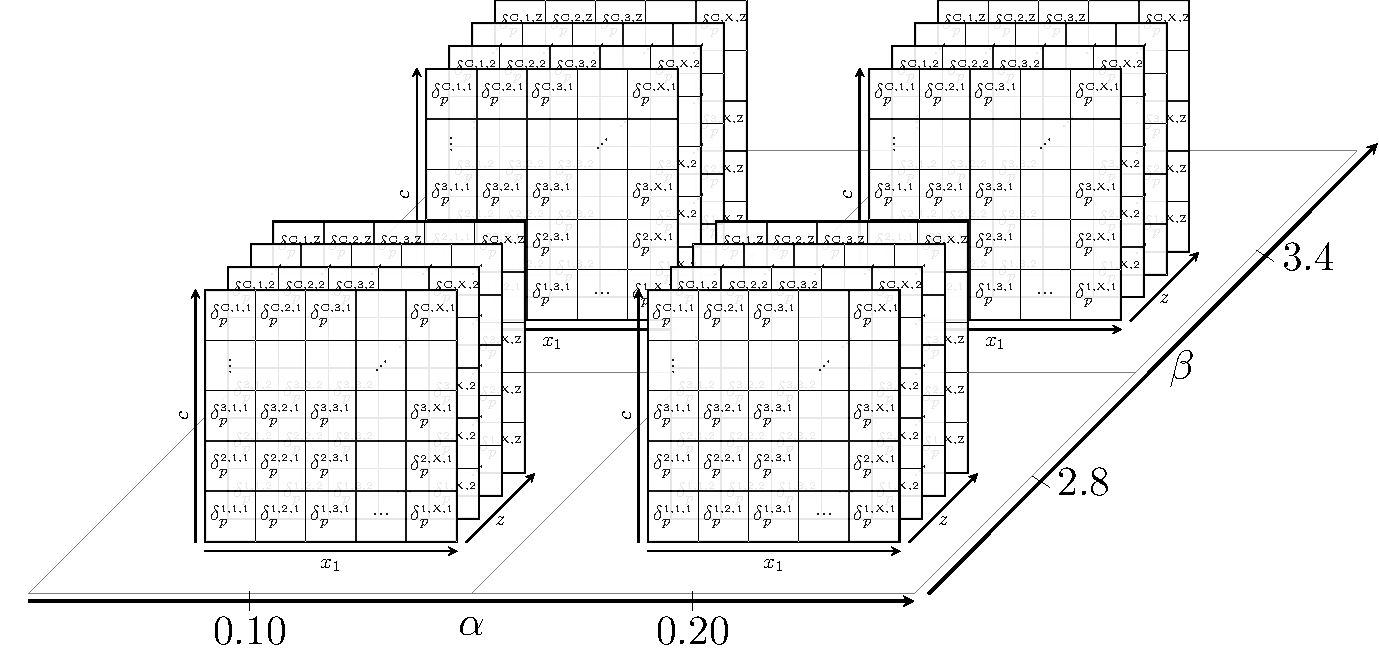
\includegraphics[width=.8\linewidth]{matrices_cube.pdf}
    \caption[Schéma de fonctionnement de la correction de biais à 5 dimensions
    de la méthode \bbc5D]{Schéma de fonctionnement de la correction de biais à 5
        dimensions de la méthode \bbc5D~: les paramètres $\alpha$ et $\beta$
        sont générés sur une grille de taille $2\times2$, et à chacune des
        valeurs de cette grille sont associées les matrices de découpe de
    l'échantillon BiasCor en 3 dimensions~: $x_1$, $c$ et $z$. Les valeurs
finales à ajouter au module de distance de la SN simulée résulte de
l'interpolation en 5D du meilleur ajustement.}
    \label{fig:mat5D}
\end{figure}

Les valeurs finales de correction sont les interpolations en 3 dimensions de
$\delta\mu_{\rm biais}$ à chaque valeur de $\alpha$ et $\beta$ pour chaque
itération de l'ajustement \bbc, dont les résultats sont également interpolés
linéairement. Une fois ces valeurs corrigées, $\alpha$, $\beta$, $\gamma_{\rm
env}$, $M_{z_i}$ et $\sigma_{\mu}$ sont minimisés par \saltmu, et l'ajustement
de $M_{z_i}$ en fonction du redshift par \wfit\ donne les valeurs des paramètres
cosmologiques. Ce fonctionnement est résumé Figure~\ref{fig:bbc5d}.

\begin{figure}[]
    \centering
    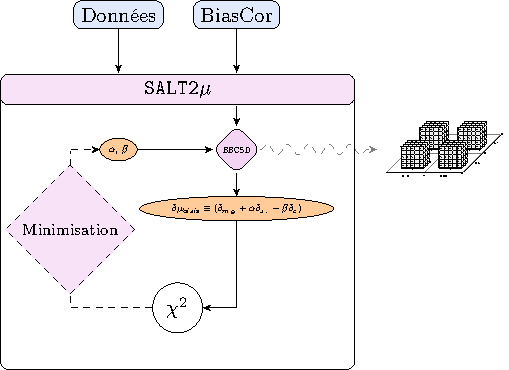
\includegraphics[scale=2]{bbc5D.pdf}
    \caption[Schéma de fonctionnement de la méthode de correction de biais de
    \bbc5D]{Schéma de fonctionnement de la méthode de correction de biais de
        \bbc\ lorsqu'elle est dans sa version à 5 dimensions. Contrairement à
        \bbc1D, ici l'ajustement de $\alpha$ et $\beta$ se fait en même temps
        que la correction de biais, cette dernière étant dépendante des valeurs
        des premières. Les valeurs de $\delta\mu_{\rm biais}$ à ajouter à $\mu$
        \textbf{et} de $\alpha$ et $\beta$ sont les interpolations du meilleur
        ajustement, donnant en sortie des $M_{z_i}$ qui permettent l'ajustement
    par \wfit.}
    \label{fig:bbc5d}
\end{figure}

\subsection{\bbc7D}\label{ssec:bbc7D}

Dans les travaux de~\cite{smith2020}, il a été déterminé que le paramètre
$\gamma_{\rm env}$ ajusté par \bbc5D présentait un biais si l'échantillon
analysé avait des corrélations entre les paramètres d'étirement et/ou de couleur
avec la masse de la galaxie hôte. Pour prendre en compte ces biais dans la
\textit{mass step},~\cite{popovic2021a} ont alors introduit deux nouvelles
dimensions au terme $\delta\mu_{\rm biais}$ de l'Équation~\ref{eq:mu5D}~:
$\theta$, un décalage de magnitude générique, et $M_*$ la masse de la galaxie
hôte.

L'idée de cet ajout est d'attribuer un décalage de magnitude de $+\theta$ à une
moitié \textit{aléatoire} de l'échantillon BiasCor, et $-\theta$ à l'autre
moitié~; ce paramètre, complètement décorrélé des propriétés environnementales,
est donc par essence différent de $\gamma_{\rm env}$, et permet une plus grande
flexibilité que d'utiliser $\delta\mu_{\rm env} = \pm\gamma_{\rm env}/2$ pour
$X_* \gtrless S$, respectivement.

Ces paramètres sont utilisés à chaque étape de l'ajustement \bbc, passant d'un
$\delta\mu_{\rm biais}$ en 5 dimensions ($\overrightarrow{x_5} = \{z, x_1, c,
\alpha, \beta\}$) à 7 dimensions $\{\overrightarrow{x_5}, \theta, M_*\}$.
$\delta\mu_{\rm biais}$ est interpolé pour les six premières, et évalué dans des
intervalles selon $M_*$. Les valeurs $\delta\mu_{\rm env}$ permettent
l'interpolation de l'échantillon BiasCor entre $\pm\theta$ suivant~:
\begin{equation}
    \delta\mu_{\rm biais} =
    f\times\delta\mu_{\rm biais}(\overrightarrow{x_5}, +\theta, M_*)
    + (1-f)\times\delta\mu_{\rm biais}(\overrightarrow{x_5}, -\theta, M_*)
\end{equation}
avec $\DS f = \frac{\delta\mu_{\rm env}+\theta}{2\theta}$. $\theta$ étant
indépendant des paramètres de SNe, il permet d'examiner des corrélations entre
n'importe quelle propriété de galaxie hôte et la magnitude des SNe~Ia.

C'est avec ce formalisme de \bbc\ que nous traitons nos simulations dans le
chapitre suivant, dans lequel nous répertorions les corrélations que nous
voulons tester et créons pour ce faire nos propres \hostlib\ où l'étirement est
donné par le modèle du Chapitre~\ref{ch:stretch} et publié
dans~\cite{nicolas2021}.

\clearpage

\thispagestyle{plain}
% \vspace*{-3cm}
\vfill
\minilof
\vfill
\minilot
\vfill

% \bibliographystyle{../main/aa_url}
% \shorthandoff{:}
% \bibliography{../chapters/99_references}

\end{document}
